\documentclass{beamer}
\usepackage[english]{babel}
\usepackage[utf8]{inputenc}

\usetheme{Madrid}
\usecolortheme{default}
\useinnertheme{circles}

\usepackage{xcolor}
\usepackage{hyperref}
\definecolor{links}{HTML}{0000FF}
\hypersetup{colorlinks, urlcolor = links}
\usepackage[
    backend=biber,
    style=alphabetic,
    sorting=ynt
]{biblatex}
\addbibresource{references.bib}
\usepackage{graphicx} % Allows including images
\usepackage{booktabs} % Allows the use of \toprule, \midrule and \bottomrule in tables
\usepackage{graphicx}
\usepackage{wrapfig}
\usepackage{listings}
\usepackage{pythonhighlight}
\graphicspath{{./images/}}

\beamertemplatenavigationsymbolsempty

%------------------------------------------------------------
%This block of code defines the information to appear in the
%Title page
\title[\textcolor{white}{Forecasting BSE SENSEX and S\&P-500}] %optional
{Forecasting S\&P BSE SENSEX and S\&P-500 Indices Using ARIMA and Prophet}

% \subtitle{And its subtitle}

\author[Suraj Prakash Sharma] % (optional)
{Suraj Prakash Sharma \newline (BLENP2DSC20038)}

\institute[] % (optional)
{
  M.Tech Data Science (IInd Semester)\\
  Amrita Vishwa Vidyapeetham, School of Engineering, Bengaluru
}

\date[] % (optional)
{Project Presentation, May 2021}

%End of title page configuration block
%------------------------------------------------------------



%------------------------------------------------------------
%The next block of commands puts the table of contents at the 
%beginning of each section and highlights the current section:

%------------------------------------------------------------

\begin{document}
%The next statement creates the title page.
\frame{\titlepage}

%---------------------------------------------------------
%This block of code is for the table of contents after
%the title page
\begin{frame}
	\frametitle{Table of Contents}
	\tableofcontents
\end{frame}
%---------------------------------------------------------
%Changing visivility of the text
\section{Objective \& Problem Statement}
\begin{frame}{Objective \& Problem Statement}
	\begin{block}{Objective}
		Forecasting S\&P BSE SENSEX and S\&P-500 Using Autoregressive Integrated Moving Average (ARIMA) \& Prophet Library.
	\end{block}
	\pause
	\begin{block} {Problem Statement}
		\begin{itemize}
			\item There are several studies in the research community which were carried out on the predictions of stock market returns using ARIMA and other powerful models especially for developed markets i.e. USA, European Markets. However very few have focused on emerging/developing and less developed markets.
			\item This study fills the gap by forecasting S\&P BSE SENSEX (Emerging Market Index) and S\&P-500 (Developed Market Index) in order to help the investors to make a more informed decision related to their investments regarding both the markets.
		\end{itemize}
	\end{block}
\end{frame}

%---------------------------------------------------------

\section{Literature Review}
\begin{frame}{Literature Review}
	\begin{itemize}
		\item Forecasting stock market returns plays a pivotal role whenever an investor/investment firm/organisation wants to build an investment strategy/policies \cite{challa_malepati_kolusu_2020}.
		      \pause
		\item Computational advancements have led to various econometric models which have been used consistently to anticipate market movements/irregularities and thus forecast the future prices/returns.
		      \pause
		\item ARIMA and its variants are one kind of time series models which can be used for short-term forecasting of financial time series data and various studies done in the research community uses ARIMA or variants of ARIMA models to forecast econometric variables like GDP, CPI, HPI, or price of an indexed financial assets etc.
		      \pause
		\item The Jenkins ARIMA approach is more efficient then other econometric models which are based on regression and exponential smoothing.
	\end{itemize}
\end{frame}

\begin{frame}{Different Types of Markets \cite{10.2307/2325486}}
	\begin{itemize}
		\item There are various studies done by prominent economists like Paul Samuelson, Mandelbrot about the nature of the market but it was Eugene Fama \cite{10.2307/2325486} who gave a framework to classify the nature of the market in his influential $1970$ paper where he discussed his famous, controversial theory known as Efficient Market Hyphothesis.
		      \pause
		\item Efficient Market Hyphothesis (EMH): It states that the price of any financial asset or product at any time reflects all the public and private information which the market has processed.
		      \pause
		\item Direct conclusion of EMH is that it is impossible to beat the market consistently (i.e. generate alpha ($\alpha$)).
		      \pause
		\item According to EMH there are $3$ types of tests proposed to categorize the markets: 1. Weak Form (Dependent only on historical prices), 2. Semi-Strong (Depends on publicly available information i.e. annoucements of annual earnings, stock splits etc), 3. Strong Form (Depends on private information about the asset i.e. insider trading etc).
	\end{itemize}
\end{frame}
%---------------------------------------------------------

% \section{Second section}

%---------------------------------------------------------
\section{Datasets \& Methodology}
\begin{frame}{Datasets \& Methodology}
	\begin{itemize}
		\item The datasets are collected using either the library or by \href{https://cutt.ly/5b6Yn9L}{Yahoo Finance website}.
	\end{itemize}
	\begin{table}
		\begin{tabular}{c l c l}
			\toprule
			\textbf{Sr.No} & \textbf{Dataset Name} & \textbf{Time-Period} & \textbf{Source}       \\
			\midrule
			1              & S\&P BSE SENSEX       & 2000-2020            & quandl library        \\
			2              & India VIX             & 2008-2020            & investpy library      \\
			3              & S\&P-500              & 2000-2020            & Yahoo Finance Website \\
			4              & CBOE VIX              & 1990-2020            & investpy library      
			\bottomrule
		\end{tabular}
		\caption{Source of Datasets.}
	\end{table}
	\begin{itemize}
		\item India VIX \& CBOE VIX Index datasets are used for explaining the market volatility which was high during the year 2007-2008 \& same kind of volatility was also observed in the year 2020-2021.
	\end{itemize}
\end{frame}

\section{Exploratory Data Analysis (EDA)}
\begin{frame}{Exploratory Data Analysis (EDA)}
	\begin{itemize}
		\item There are various kinds of interactive plots which were created in order to understand the datasets clearly before developing time series based models.
		      \pause
		\item This section is divided into two parts:
		      \begin{itemize}
		      	\item S\&P BSE SENSEX Index EDA.
		      	\item S\&P-500 Index EDA.
		      \end{itemize}
	\end{itemize}
\end{frame}

\begin{frame}{Descriptive Statistics of S\&P BSE SENSEX}
	\begin{table}[htbp]
		\centering
		\begin{tabular}{c c c c}
			\textbf{Sr.No} & \textbf{Stats}         & \textbf{Close} & \textbf{\%-Change} \\
			\toprule
			1              & Mean                   & 17930.2        & 0.0525427          \\
			2              & Median                 & 17222.6        & 0.0952336          \\
			3              & Min                    & 2600.12        & -13.1526           \\
			4              & Max                    & 47751.3        & 17.3393            \\
			5              & Std. Dev               & 11379.9        & 1.4641             \\
			6              & Skewness               & 0.401981       & -0.13972           \\
			7              & Kurtosis               & -0.875044      & 9.65161            \\
			8              & Jarque Bera Test$^{*}$ & (307.514, 0.0) & (20257.592, 0.0)   \\
			\bottomrule
		\end{tabular}
		\caption{Descriptive Statistics of S\&P BSE SENSEX Close and \%-Change Values.}
		\label{tab:my_label}
	\end{table}
	$*$ \href{https://cutt.ly/5nwffCF}{Jarque Bera Test} is used to find out whether the values are normally distributed or not.
\end{frame}

\begin{frame}{S\&P BSE SENSEX EDA: Line Plot (2000-2020)}
	\begin{figure}
		\centering
		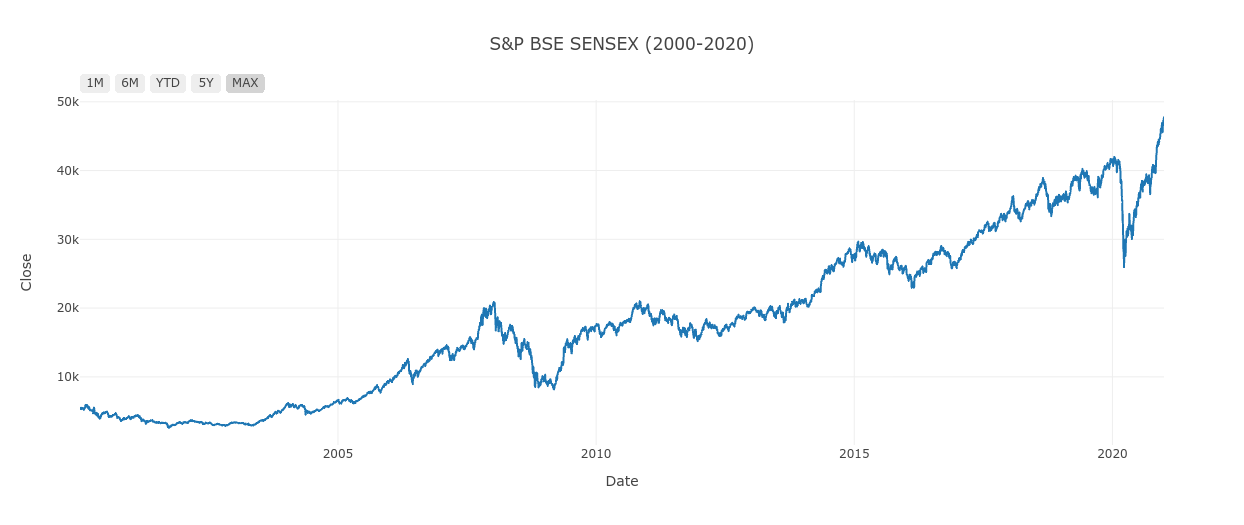
\includegraphics[width = \textwidth]{SENSEX 2000-2020 Line Plot-1}
		\caption{S\&P BSE SENSEX Line Plot.}
		\label{fig:my_label}
	\end{figure}
\end{frame}
\begin{frame}{S\&P BSE SENSEX EDA: Simple Moving Average \& Yearly Distribution Plot}
	\begin{figure}
		\centering
		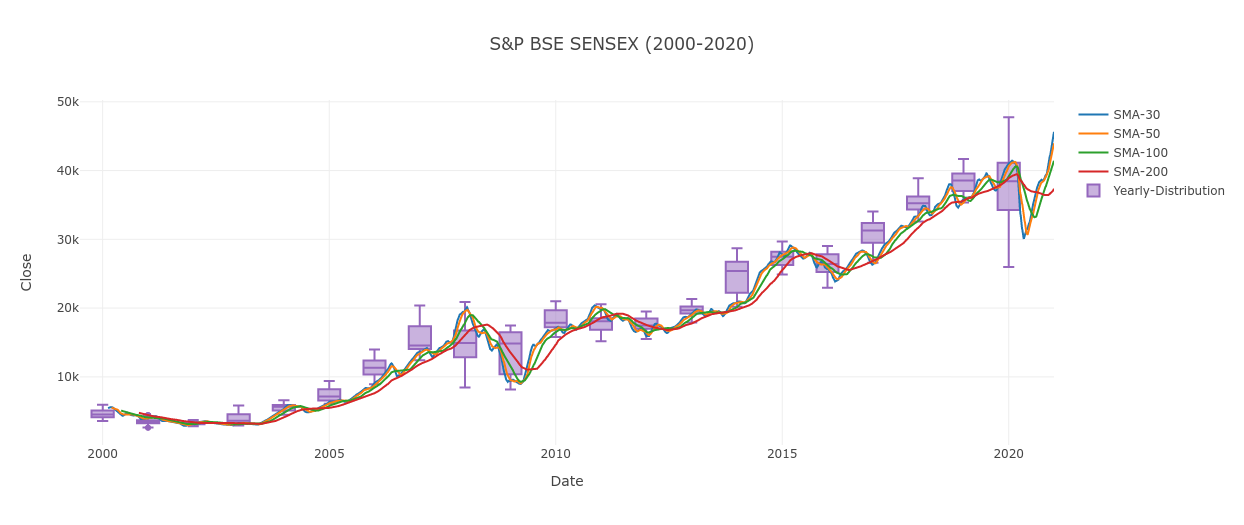
\includegraphics[width = \textwidth]{images/SENSEX 2000-2020 Line Plot-2}
		\caption{S\&P BSE SENSEX Simple Moving Average (30, 50, 100, 200) and Yearly Distribution}
		\label{fig:my_label}
	\end{figure}
\end{frame}

\begin{frame}{S\&P BSE SENSEX EDA: \%-Change Plot}
	\begin{figure}
		\centering
		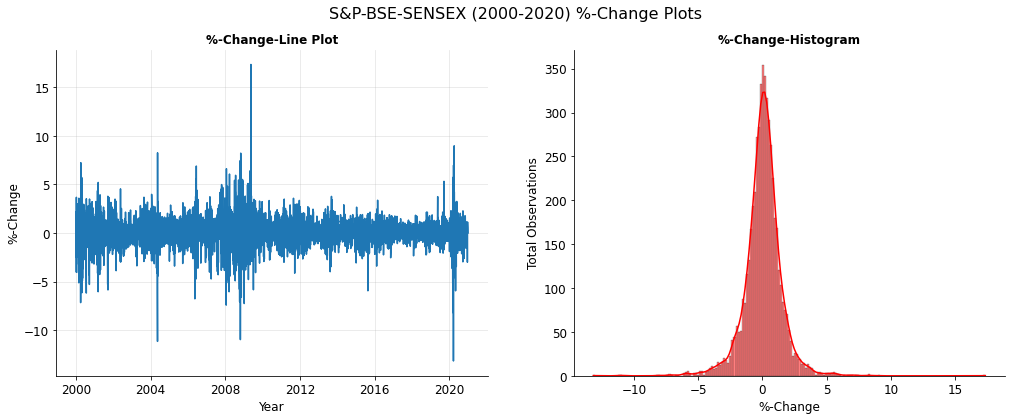
\includegraphics[width = \textwidth]{images/SENSEX 2000-2020 Change Plot}
		\caption{\%-Change Plot in the Value of S\&P BSE SENSEX.}
		\label{fig:my_label}
	\end{figure}
\end{frame}

\begin{frame}{Descriptive Statistics of S\&P-500 Index}
	\begin{table}[htbp]
		\centering
		\begin{tabular}{c c c c}
			\textbf{Sr.No} & \textbf{Stats}         & \textbf{Close} & \textbf{\%-Change} \\
			\toprule
			1              & Mean                   & 1653.27        & 0.025695           \\
			2              & Median                 & 1386.95        & 0.0593618          \\
			3              & Min                    & 676.53         & -11.9841           \\
			4              & Max                    & 3735.36        & 11.58              \\
			5              & Std. Dev               & 673.836        & 1.25313            \\
			6              & Skewness               & 1.03217        & -0.1538            \\
			7              & Kurtosis               & 0.0629593      & 10.736             \\
			8              & Jarque Bera Test$^{*}$ & (938.363, 0.0) & (25339.385, 0.0)   \\
			\bottomrule
		\end{tabular}
		\caption{Descriptive Statistics of S\&P-500 Close and \%-Change Values.}
		\label{tab:my_label}
	\end{table}
	$*$ \href{https://cutt.ly/5nwffCF}{Jarque Bera Test} is used to find out whether the values are normally distributed or not.
\end{frame}

\begin{frame}{S\&P-500 EDA: Line Plot}
	\begin{figure}
		\centering
		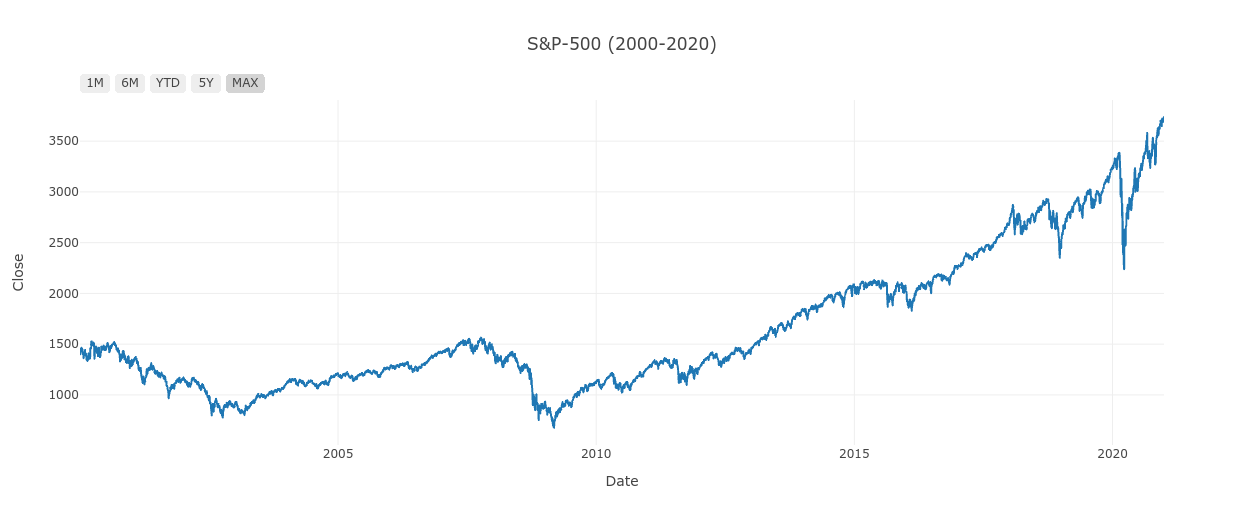
\includegraphics[width = \textwidth]{images/S&P-500 Line-Plot-1}
		\caption{S\&P-500 Line Plot}
		\label{fig:my_label}
	\end{figure}
\end{frame}

\begin{frame}{S\&P-500 EDA: Simple Moving Average \& Yearly Distribution}
	\begin{figure}
		\centering
		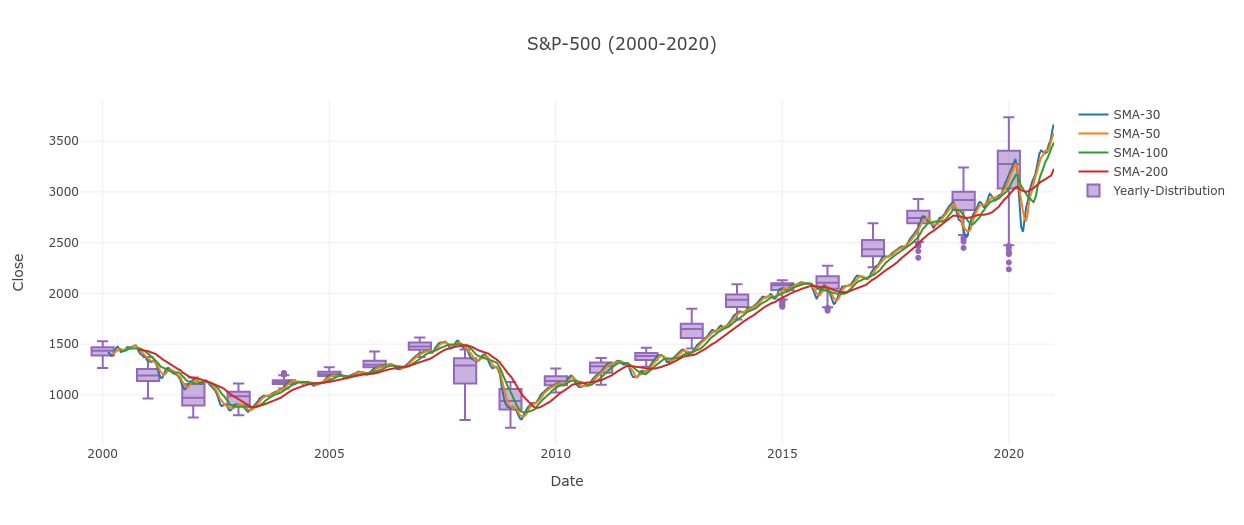
\includegraphics[width = \textwidth]{images/S&P-500 Line-Plot-2}
		\caption{S\&P-500 SMA (30, 50, 100, 200) and Yearly Distribution.}
		\label{fig:my_label}
	\end{figure}
\end{frame}

\begin{frame}{S\&P-500 EDA: \% Change Plots}
	\begin{figure}
		\centering
		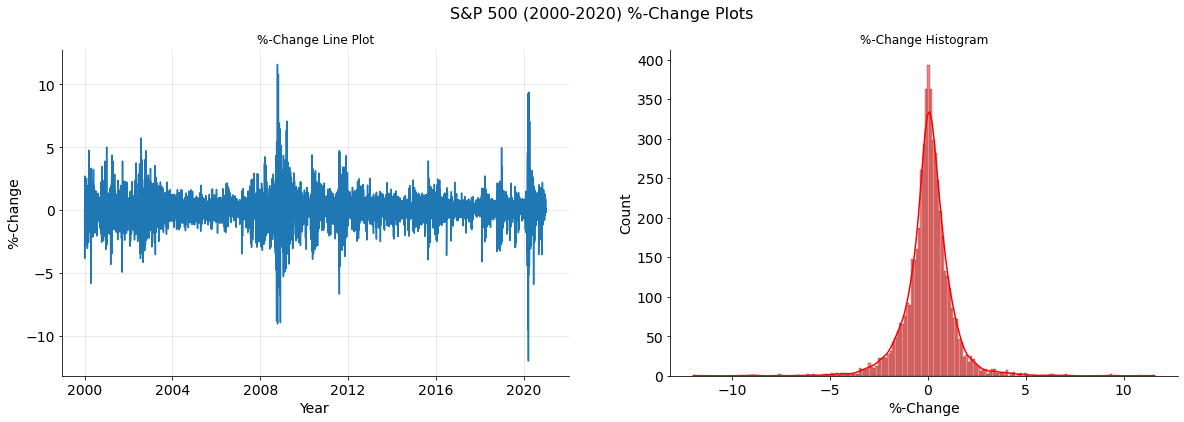
\includegraphics[width = \textwidth]{images/S&P-500 Change Plot.png}
		\caption{S\&P-500 \%-Change Plot.}
		\label{fig:my_label}
	\end{figure}
\end{frame}

\begin{frame}{Insights from EDA of S\&P BSE SENSEX and S\&P-500}
	\begin{itemize}
		\item The \%-Change plots shows the change in the value of indexes from previous day $x_{t - 1}$ to current day $x_{t}$ and it turns out that the sequence which we got is a \textbf{White Noise} with approximately $0$ mean ($\mu$) and constant standard deviation ($\sigma$) which implies that the given time series data of indexes i.e. S\&P BSE SENSEX and S\&P-500 is a \textbf{Random Walk} process hence the given time series is \textbf{non-stationary}.
		      \pause
		      \begin{figure}
		      	\centering
		      	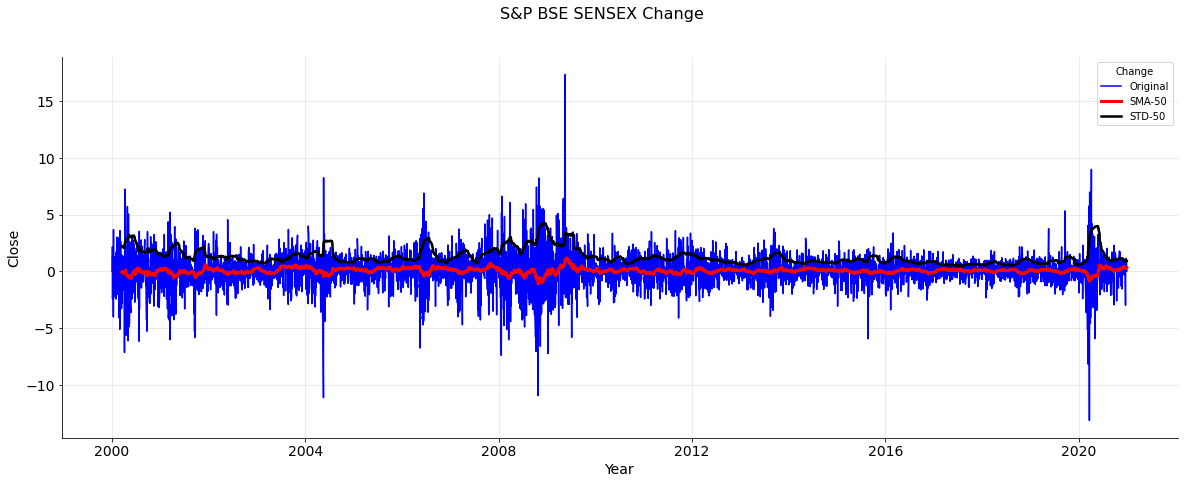
\includegraphics[width = 0.90 \linewidth]{BSE SENSEX White Noise Part}
		      	\caption{S\&P BSE SENSEX \%-Change Plot.}
		      \end{figure}
	\end{itemize}
\end{frame}

\begin{frame}{Random Walk Process Eqn's}
	\begin{figure}
		\centering
		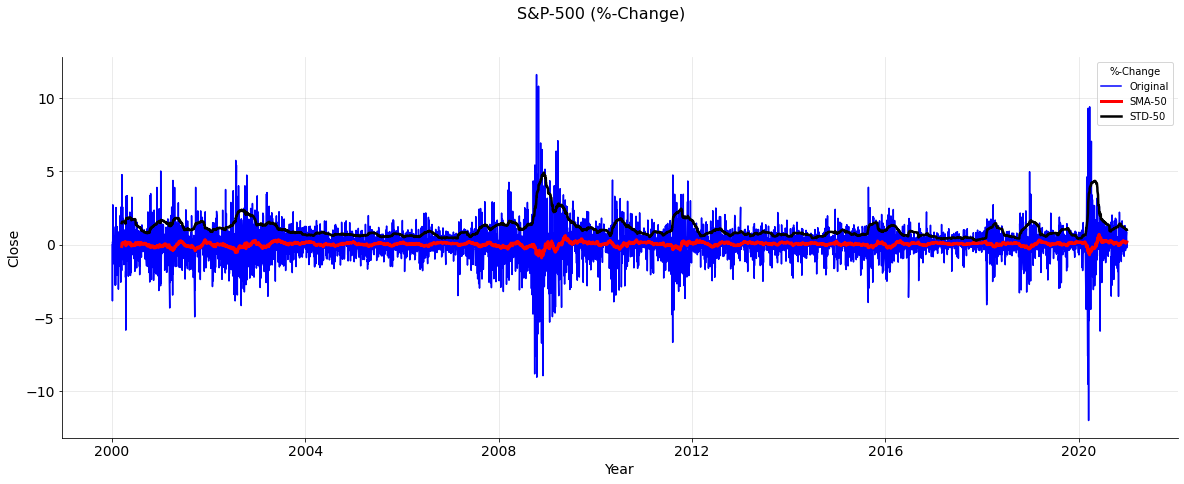
\includegraphics[width = 0.90 \linewidth]{S&P-500 White Noise Part.png}
		\caption{S\&P-500 \%-Change Plot.}
	\end{figure}
\end{frame}

\begin{frame}{Random Walk Process Eqn's}
	\begin{itemize}
		\item Random Walk Process Eqn's:  $$(i)\; P_{t} = P_{t - 1} + \epsilon_{t}$$
		      $$ (ii)\; P_{t} = d + P_{t - 1} + \epsilon_{t}$$
		      $$ (iii)\; P_{t} = P_{0} + dt + \sum_{t = 1}^{n} \epsilon_{t} $$
		      where   $P_{t} = $ Value of underlying series at time $t$. \\
		      $P_{t - 1} = $  Value of underlying series at time $t - 1$. \\
		      $d = $ Drift (which is just a trend like property for a random walk process i.e.\\ $d > 0 \implies$ Upward trend and $d < 0 \implies$ downward trend).\\
		      $\epsilon_{t} = $ White Noise or Gaussian White Noise.
	\end{itemize}
\end{frame}

\begin{frame}{INDIA VIX Index}
	\begin{figure}
		\centering
		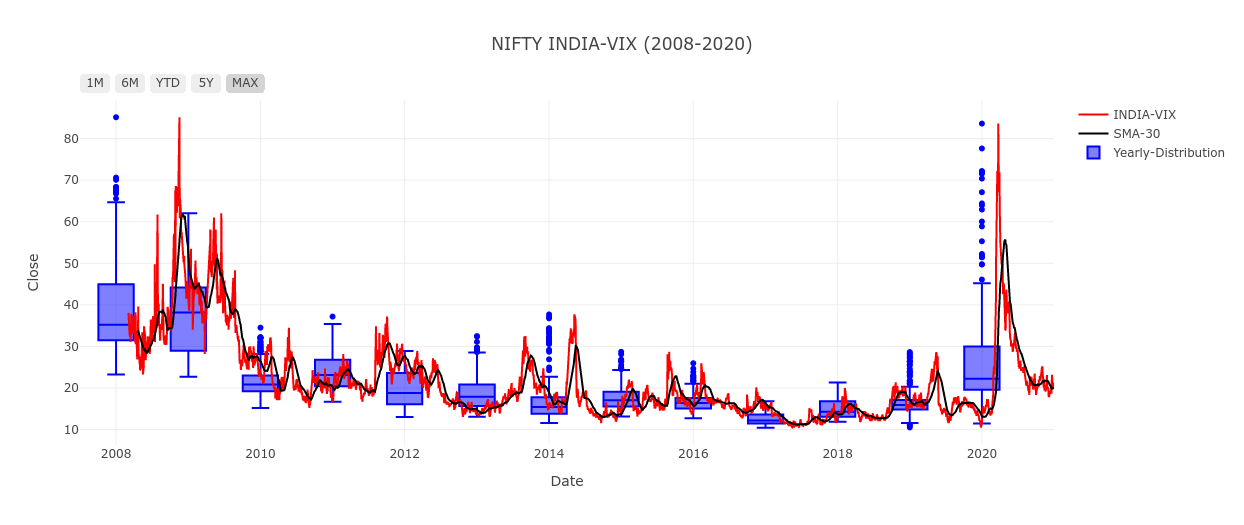
\includegraphics[width = 0.95 \textwidth]{images/INDIA-VIX-2008-2020}
		\caption{INDIA VIX (2008-2020)}
		\label{fig:my_label}
	\end{figure}
	\begin{itemize}
		\item The above plot tells us about the total volatility present in the Indian Markets from the perpective of NIFTY-50.
	\end{itemize}
\end{frame}

\begin{frame}{CBOE VIX Index}
	\begin{figure}
		\centering
		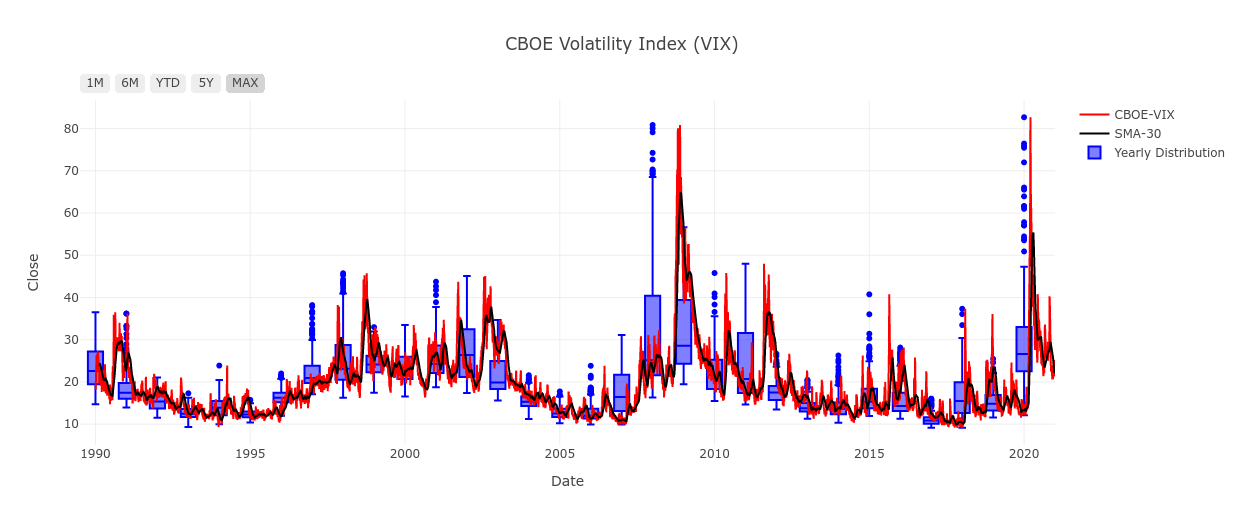
\includegraphics[width = \textwidth]{images/CBOE-VIX}
		\caption{CBOE VIX Index}
		\label{fig:my_label}
	\end{figure}
	\begin{itemize}
		\item The above figure gives us an idea about the volatility in the United States Markets from the perspective of S\&P-500.
	\end{itemize}
\end{frame}

\begin{frame}{Insights from EDA of Volatility Indexes (India VIX \& CBOE VIX)}
	\begin{itemize}
		\item The interesting insights (labelled in the figure) to note is that in the FY-2009 and FY-2021, the volatility in the market (both Indian \& United States) are pretty high beacause in the FY-2009, Global Financial Crisis happened due to crash of Mortgage market in United States and in FY-2021 COVID-19 crash happened due to great lockdown and the panic of recession.
	\end{itemize}
\end{frame}

%---------------------------------------------------------
\section{ACF, PACF, Components of Time Series}
\begin{frame}{S\&P BSE SENSEX ACF and PACF Plots}
	\begin{figure}
		\centering
		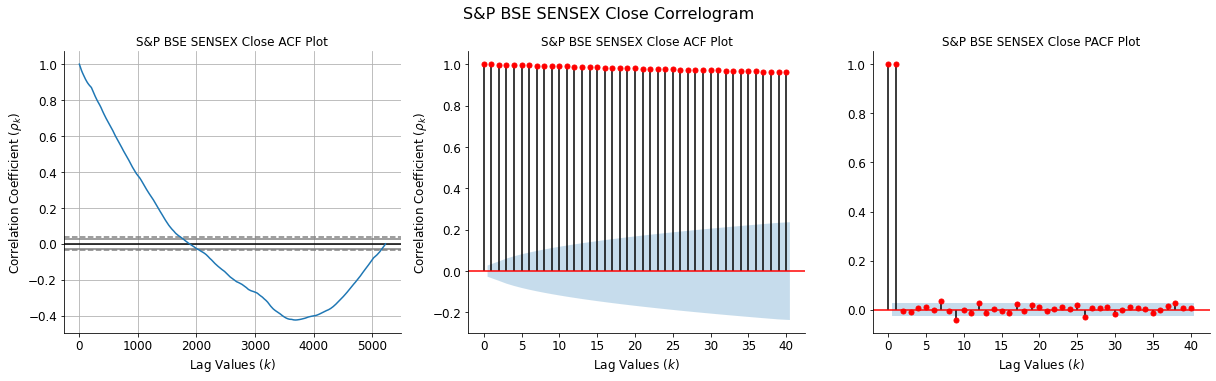
\includegraphics[width = 0.80 \textwidth]{images/SENSEX ACF and PACF Plot}
		\caption{S\&P BSE SENSEX ACF and PACF Plot.}
		\pause
		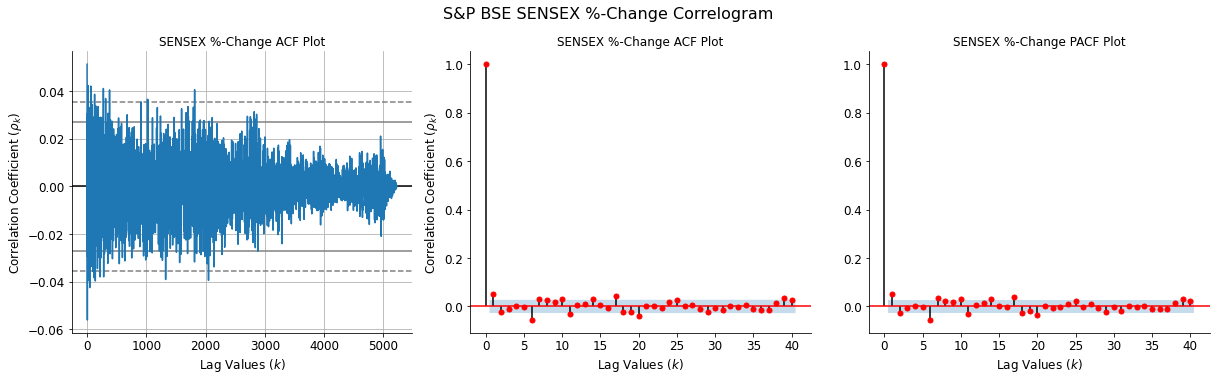
\includegraphics[width = 0.80 \textwidth]{images/SENSEX Change ACF, PACF Plots.png}
		\caption{S\&P BSE SENSEX \%-Change ACF, PACF Plot.}
	\end{figure}
		
\end{frame}

\begin{frame}{S\&P BSE SENSEX Time Series Components}
	\begin{figure}
		\centering
		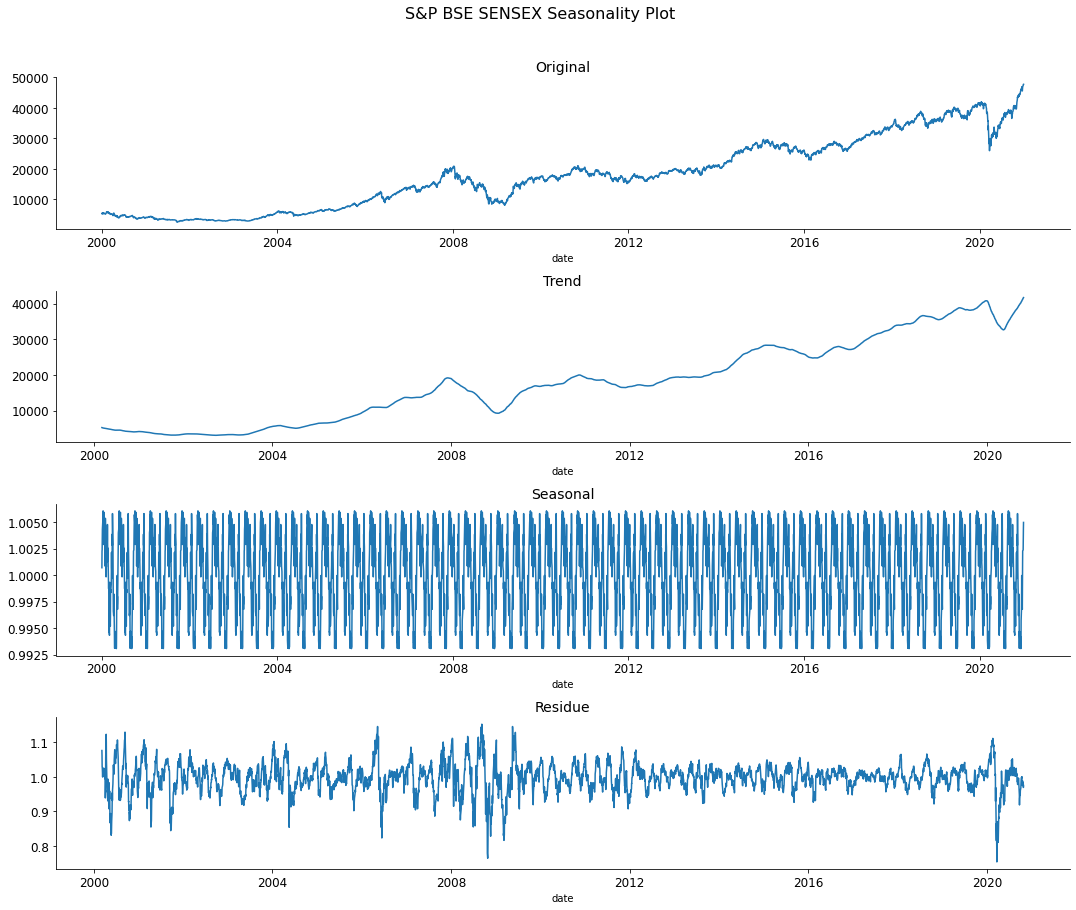
\includegraphics[width = 0.65 \textwidth]{images/SENSEX Seasonal Decompose Plot.png}
		\caption{S\&P BSE SENSEX Trend, Seasonal, Residual Plot (Quaterly).}
		\label{fig:my_label}
	\end{figure}
\end{frame}

\begin{frame}{S\&P BSE SENSEX Time Series Cyclicity Component}
	\begin{figure}
		\centering
		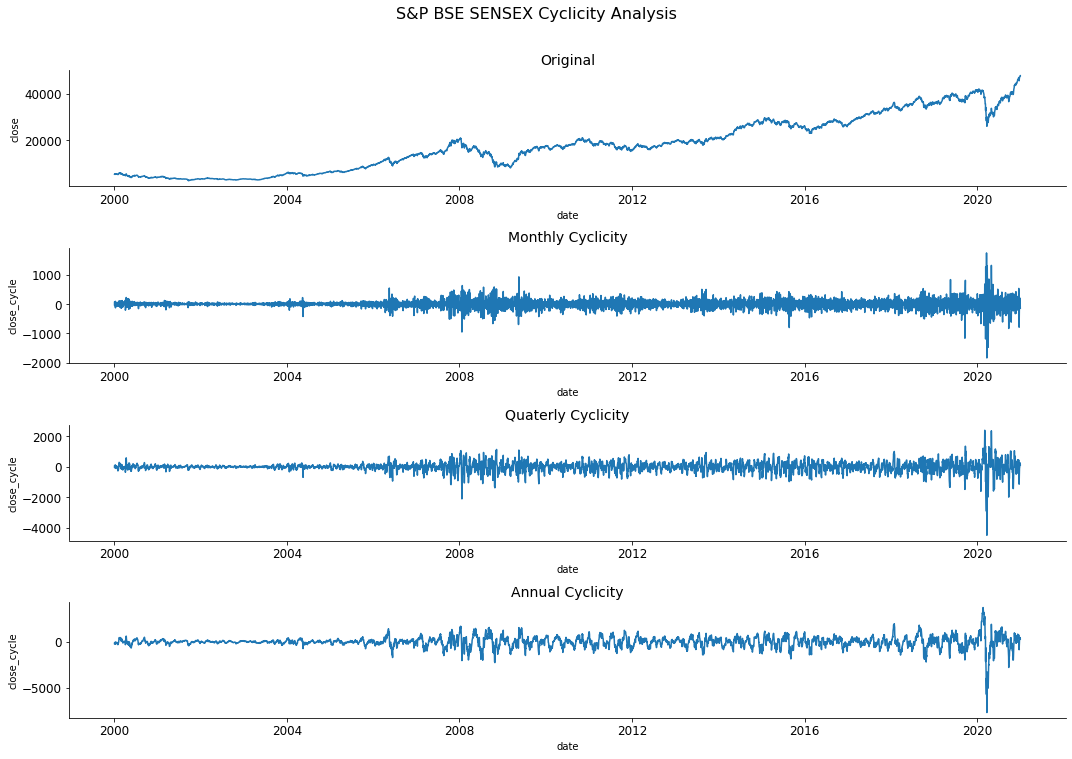
\includegraphics[width = 0.80 \textwidth]{images/SENSEX Cyclicity Plot.png}
		\caption{S\&P BSE SENSEX Montly, Quaterly and Annualy Cyclicity.}
		\label{fig:my_label}
	\end{figure}
\end{frame}

\begin{frame}{S\&P-500 ACF, PACF Plots}
	\begin{figure}
		\centering
		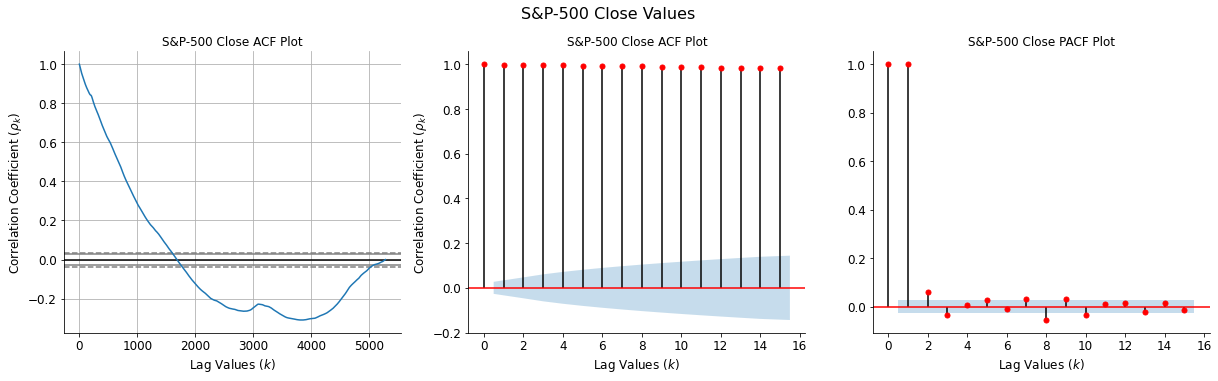
\includegraphics[width = 0.80 \textwidth]{images/S&P-500 ACF, PACF Plots.png}
		\caption{S\&P-500 ACF, PACF Plots.}
		\label{fig:my_label}
		\pause
		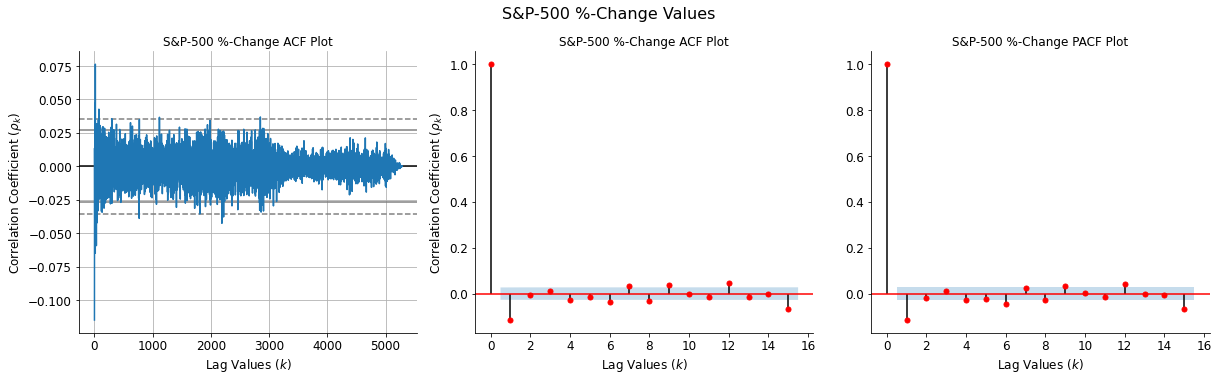
\includegraphics[width = 0.80 \textwidth]{images/S&amp;P-500 Change ACF PACF Plot.png}
		\caption{S\&P-500 \%-Change ACF, PACF Plots.}
		\label{fig:my_label}
	\end{figure}
\end{frame}

\begin{frame}{S\&P-500 Time Series Components}
	\begin{figure}
		\centering
		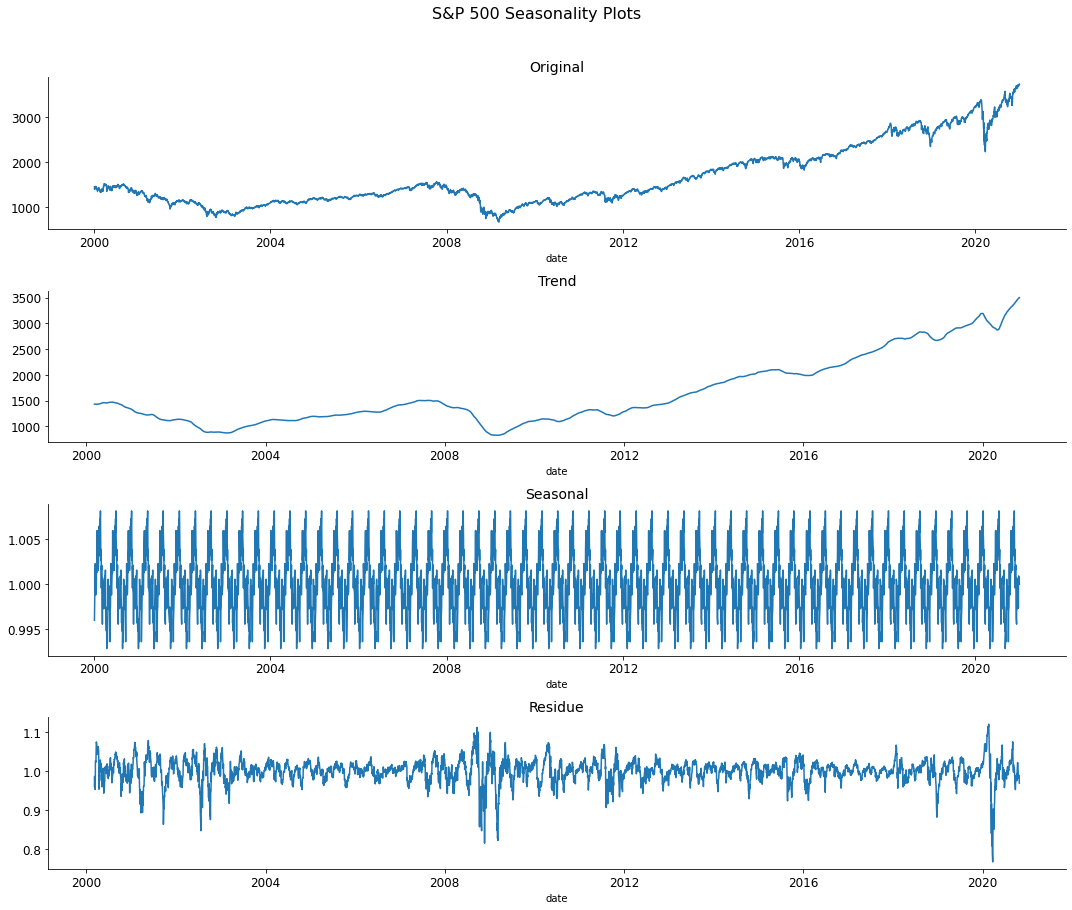
\includegraphics[width = 0.70 \textwidth]{images/S&P-500 Seasonal Decompose Plot.png}
		\caption{S\&P-500 Trend, Seasonal, Residual Plot (Quaterly).}
		\label{fig:my_label}
	\end{figure}
\end{frame}

\begin{frame}{S\&P-500 Time Series Cyclicity Component}
	\begin{figure}
		\centering
		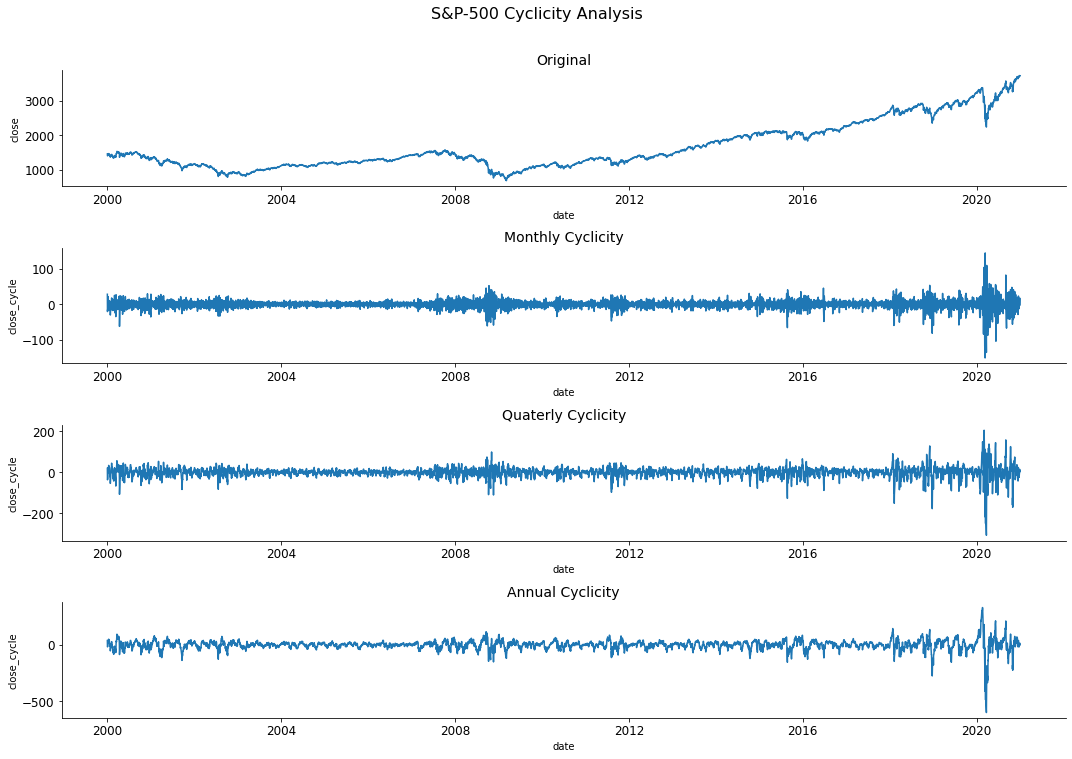
\includegraphics[width = 0.80 \textwidth]{images/S&P-500 Cyclicity Plot.png}
		\caption{S\&P-500 Montly, Quaterly and Annualy Cyclicity.}
		\label{fig:my_label}
	\end{figure}
\end{frame}

\section{Statistical Tests for Stationarity}
\subsection{Augmented Dickey Fuller Test}
\begin{frame}{Statistical Tests for Stationarity: Augmented Dickey Fuller Test}
	\begin{itemize}
		\item $H_{0}$: Given time series data is non-stationarity $\implies$ Time series data has time dependent statistical properties i.e. mean, variance, auto-correlation etc present in it.\\
		      $H_{A}:$ Given time series data is stationary $\implies$ Time series data doesn't have any time dependent statisitcal properties present in it.
		\item $p-value \le 0.05$ then we reject the $H_{0}$ otherwise we don't have enough evidence to reject the $H_{0} \implies$ failed to reject $H_{0}.$
		\item The results of ADF Test performed on both the indexes is shown on the next slide.
	\end{itemize}
\end{frame}

\begin{frame}{ADF Test Results for S\&P BSE SENSEX Index}
	\begin{table}
		\begin{tabular}{c{0.5cm} c{1cm} c c c}
			\textbf{Sr.No} & \textbf{Data} & \textbf{t-statistic} & \textbf{p-value} & \textbf{Verdict}        \\
			\midrule
			1              & Close Values  & $0.688133$           & $0.688133$       & Failed to Reject H_{0}. \\
			\bottomrule
		\end{tabular}
		\caption{S\&P BSE SENSEX Close Value ADF Test Results.}
	\end{table}
	\begin{itemize}
		\item As p-value obtained i.e. $0.998199 > 0.05 (\alpha) \implies$ Failed to Reject $H_{0} \implies$ S\&P BSE SENSEX Close values is \textbf{non-stationary}.
	\end{itemize}
	\pause
	\begin{table}[]
		\centering
		\begin{tabular}{c c c c c}
			\textbf{Sr.No} & \textbf{Data}    & \textbf{t-statistic} & \textbf{p-value}           & \textbf{Verdict} \\
			\midrule
			1              & \%-Change Values & $-16.080128$         & $5.389647 \times 10^{-29}$ & Reject H_{0}.    
			\bottomrule
		\end{tabular}
		\caption{S\&P BSE SENSEX \%-Change Values ADF Test Results.}
		\label{tab:my_label}
	\end{table}
	\begin{itemize}
		\item As p-value obtained i.e. $5.389647 \times 10^{-27} << 0.05 (\alpha) \implies$ Reject the $H_{0} \implies$ S\&P BSE SENSEX \%-Change values is \textbf{stationary}.
	\end{itemize}
\end{frame}

\begin{frame}{ADF Test Results for S\&P-500 Index}
	\begin{table}
		\begin{tabular}{c{0.5cm} c{1cm} c c c}
			\textbf{Sr.No} & \textbf{Data} & \textbf{t-statistic} & \textbf{p-value} & \textbf{Verdict}        \\
			\midrule
			1              & Close Values  & $1.631761$           & $0.99795$        & Failed to Reject H_{0}. \\
			\bottomrule
		\end{tabular}
		\caption{S\&P-500 Close Value ADF Test Results.}
	\end{table}
	\begin{itemize}
		\item As p-value obtained i.e. $0.99795 > 0.05 (\alpha) \implies$ Failed to Reject $H_{0} \implies$ S\&P-500 Close values is \textbf{non-stationary}.
	\end{itemize}
	\pause
	\begin{table}[]
		\centering
		\begin{tabular}{c c c c c}
			\textbf{Sr.No} & \textbf{Data}    & \textbf{t-statistic} & \textbf{p-value}           & \textbf{Verdict} \\
			\midrule
			1              & \%-Change Values & $-13.74109$          & $1.094051 \times 10^{-25}$ & Reject H_{0}.    
			\bottomrule
		\end{tabular}
		\caption{S\&P-500 \%-Change Values ADF Test Results.}
		\label{tab:my_label}
	\end{table}
	\begin{itemize}
		\item As p-value obtained i.e. $1.094051 \times 10^{-25} << 0.05 (\alpha) \implies$ Reject the $H_{0} \implies$ S\&P-500 \%-Change values is \textbf{stationary}.
	\end{itemize}
\end{frame}

\section{Estimating Parameters of ARIMA models \& Forecasting Using ARIMA}
\begin{frame}{Estimating Parameters of ARIMA Model i.e. SARIMAX \& Forecasting Using SARIMAX}
	\begin{figure}
		\centering
		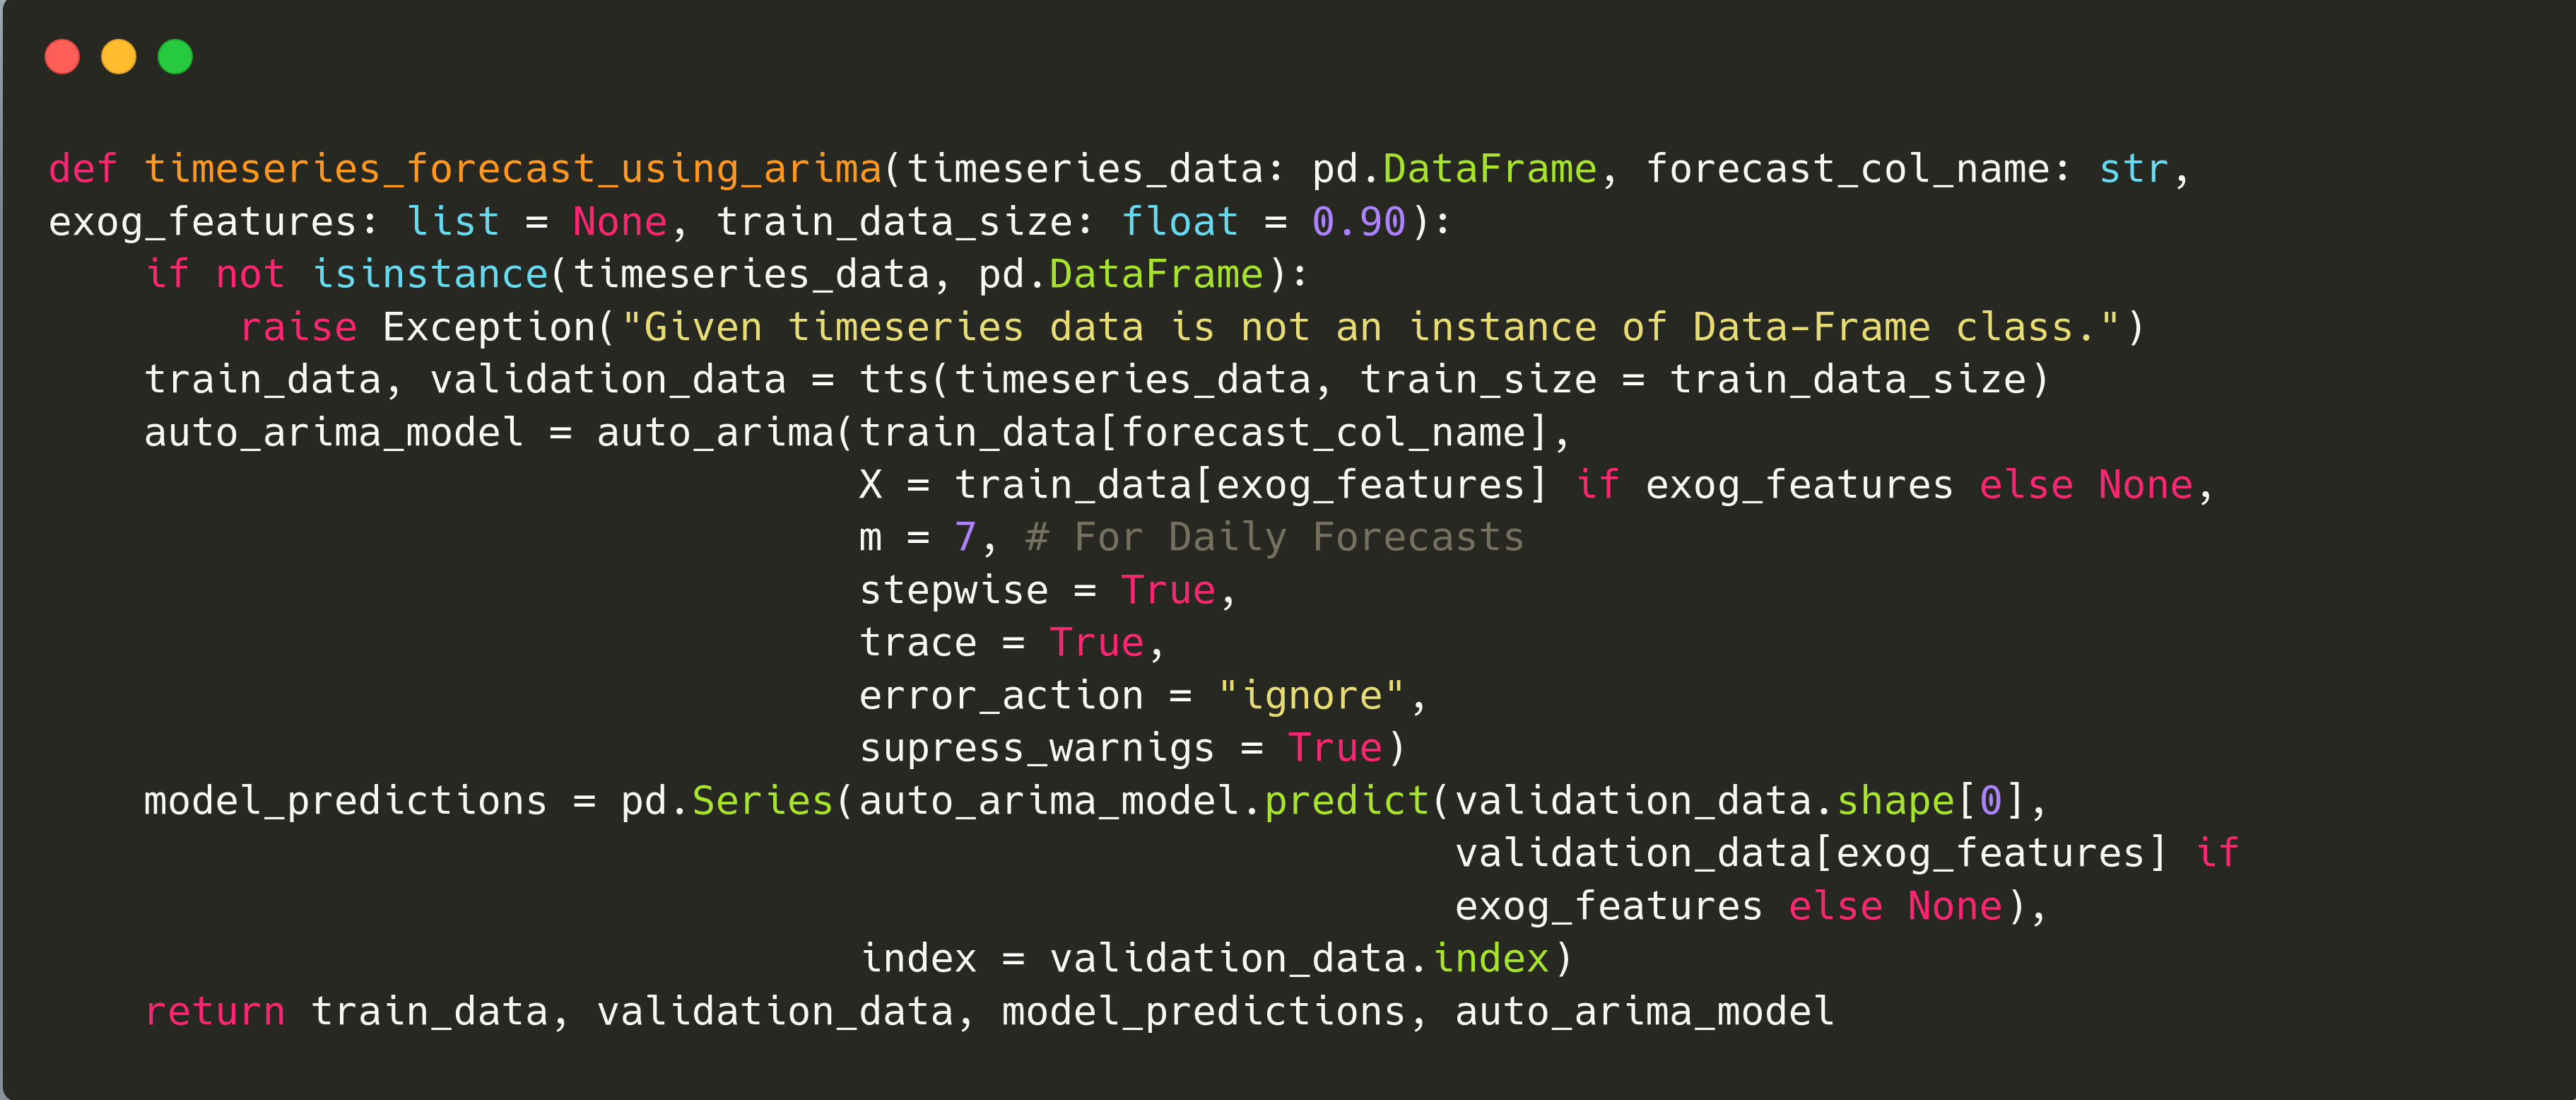
\includegraphics[width = 0.90 \textwidth]{images/timseries_forecast_using_arima.png}
		\caption{Source Code for Estimating Parameters and Forecasting Using SARIMAX.}
		\label{fig:my_label}
	\end{figure}
\end{frame}

\section{Prophet Based Training \& Forecasting}
\begin{frame}{Prophet Based Forecasting}
	\begin{figure}
		\centering
		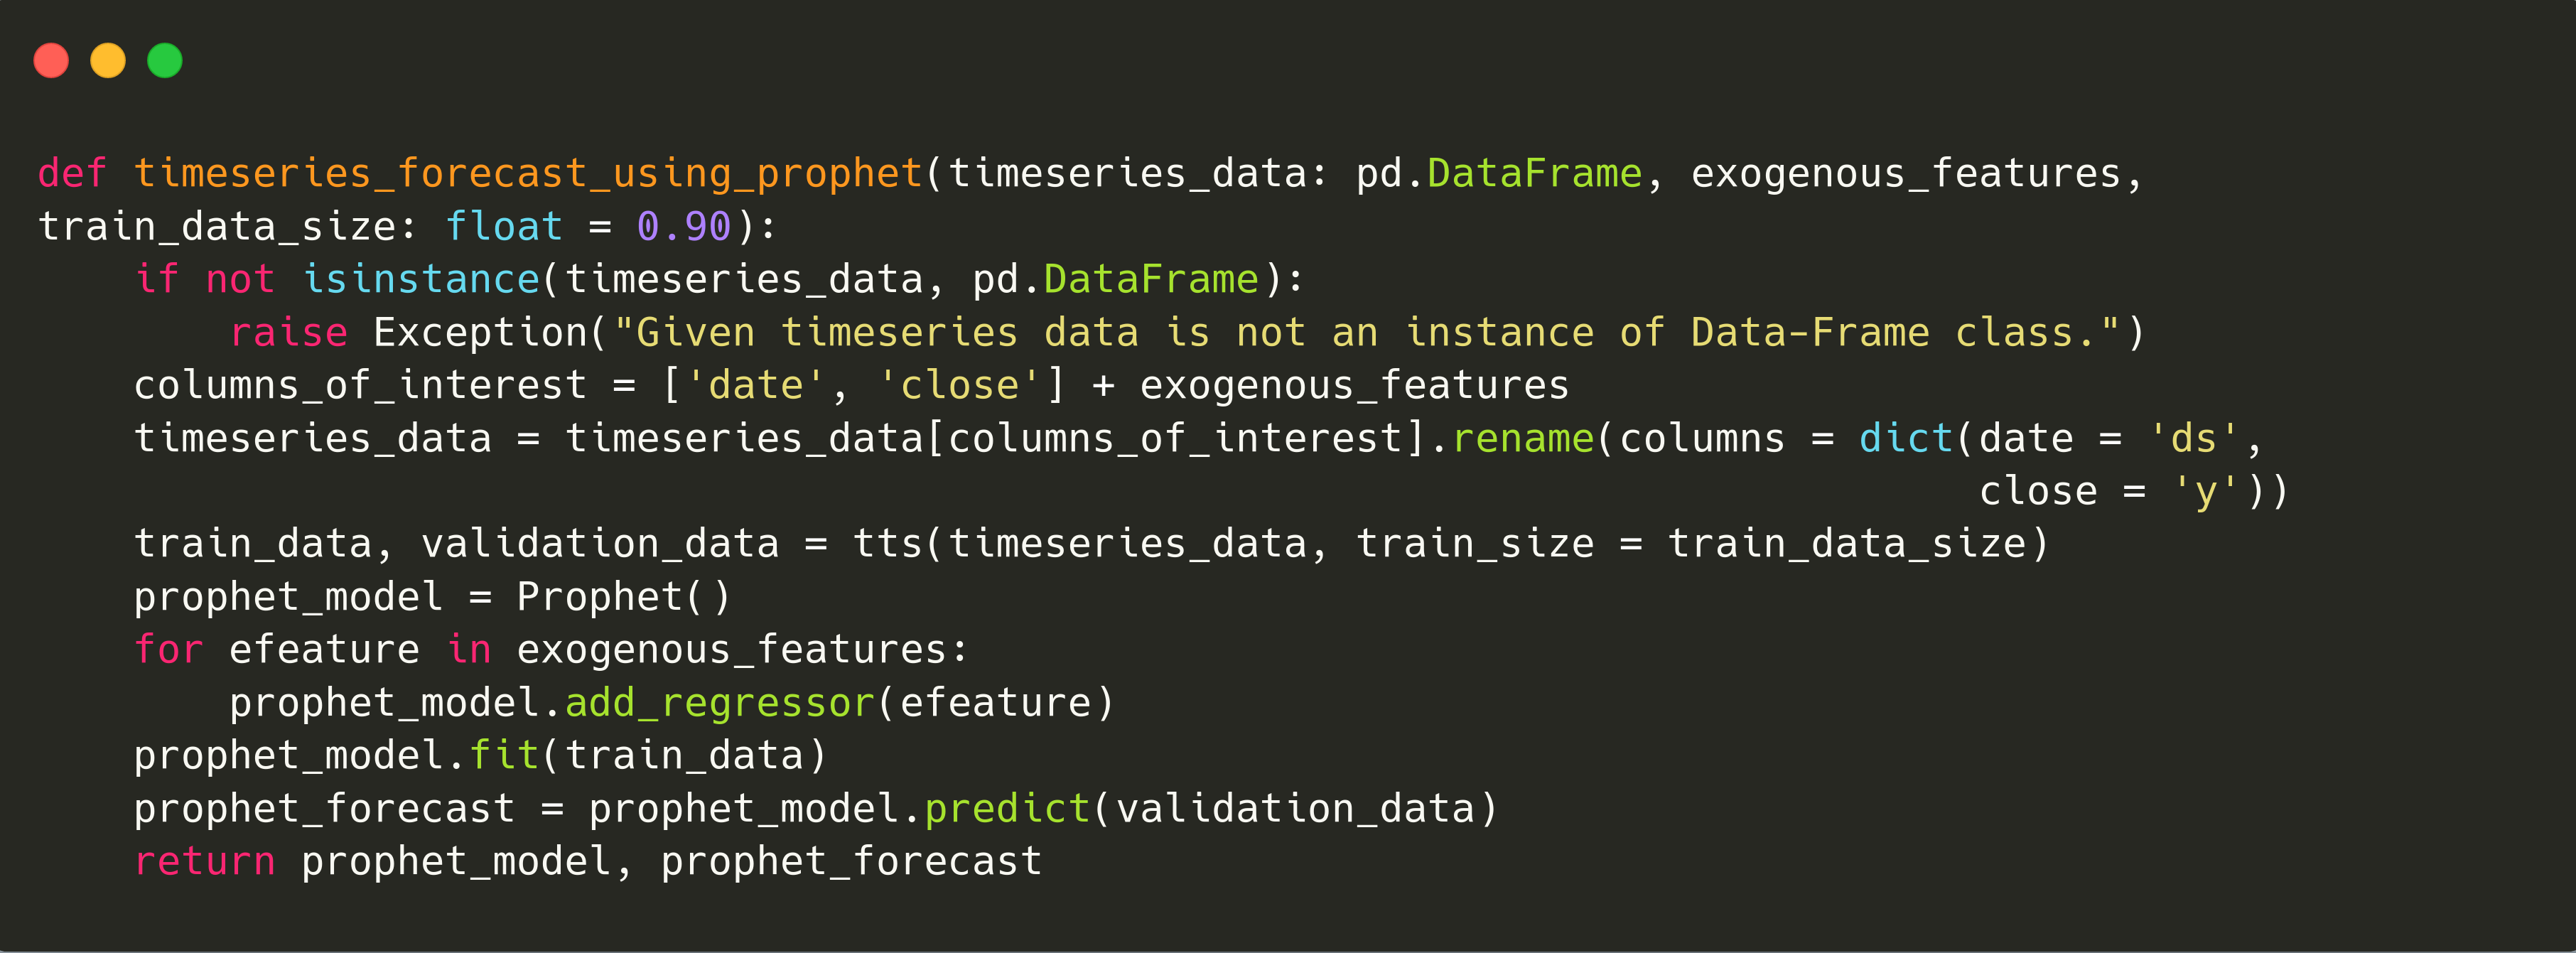
\includegraphics[width = \textwidth]{images/timeseries_forecasting_using_prophet.png}
		\caption{Source Code for Forecasting Using Prophet.}
		\label{fig:my_label}
	\end{figure}
\end{frame}

\begin{frame}{Parameters of SARIMAX Model for S\&P BSE SENSEX}
	\begin{itemize}
		\item The model used is SARIMA but as we are also exposing the SARIMA model to exogenous features i.e. those features which are not used to fit the model but have an influence on the model forecast. Hence the model used is SARIMAX where X is for exogeneous features presence.
		      \pause
		\item Estimated hyperparameters of SARIMAX $(p, d, q) \times (P, D, Q, M)$ are: \textbf{SARIMAX $(2, 0, 1) \times (2, 0, 0, 7)$} with an AIC $=63798.806$.
	\end{itemize}
	\begin{figure}
		\centering
		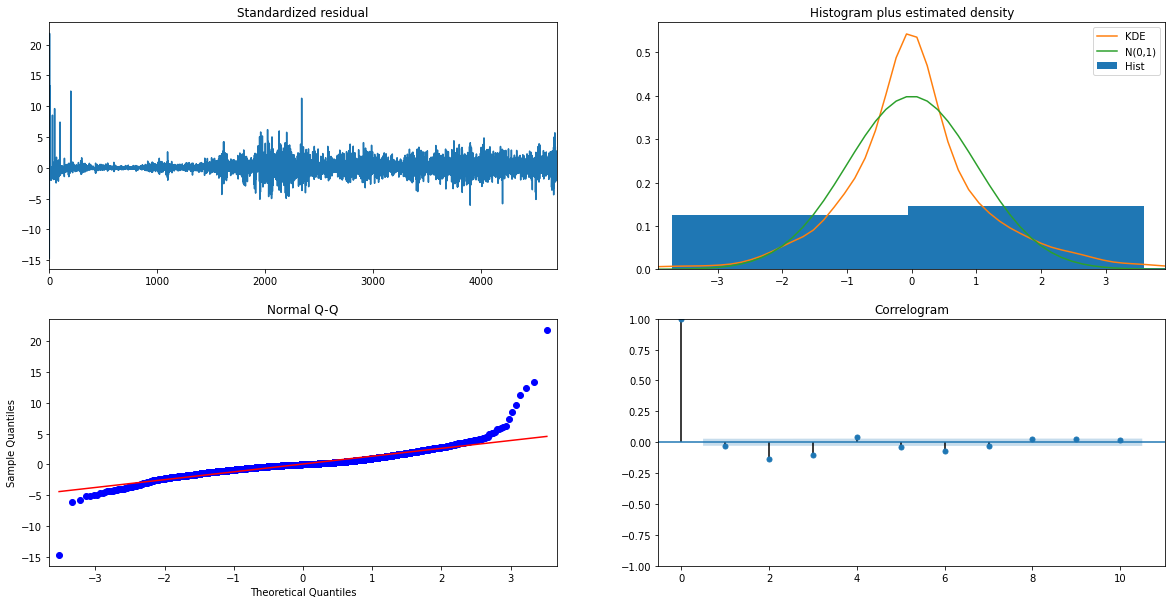
\includegraphics[width = 0.75 \textwidth]{images/SENSEX Auto ARIMA Training Results}
		\caption{}
		\label{fig:my_label}
	\end{figure}
\end{frame}

\begin{frame}{SARIMAX Performance on Validation Set (S\&P BSE SENSEX)}
	\begin{figure}
		\centering
		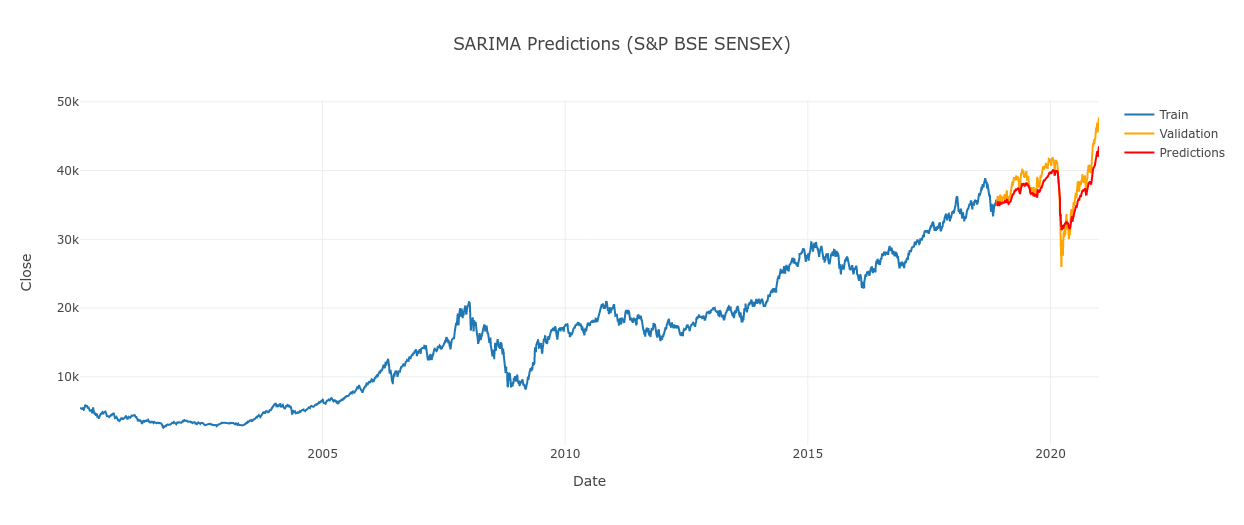
\includegraphics[width = \textwidth]{images/SARIMA-SENSEX-Predictions.png}
		\caption{SARIMA Model Predictions for Validation Data (S\&P BSE SENSEX).}
		\label{fig:my_label}
	\end{figure}
\end{frame}

\begin{frame}{Prophet Performance on Validation Set (S\&P BSE SENSEX)}
	\begin{figure}
		\centering
		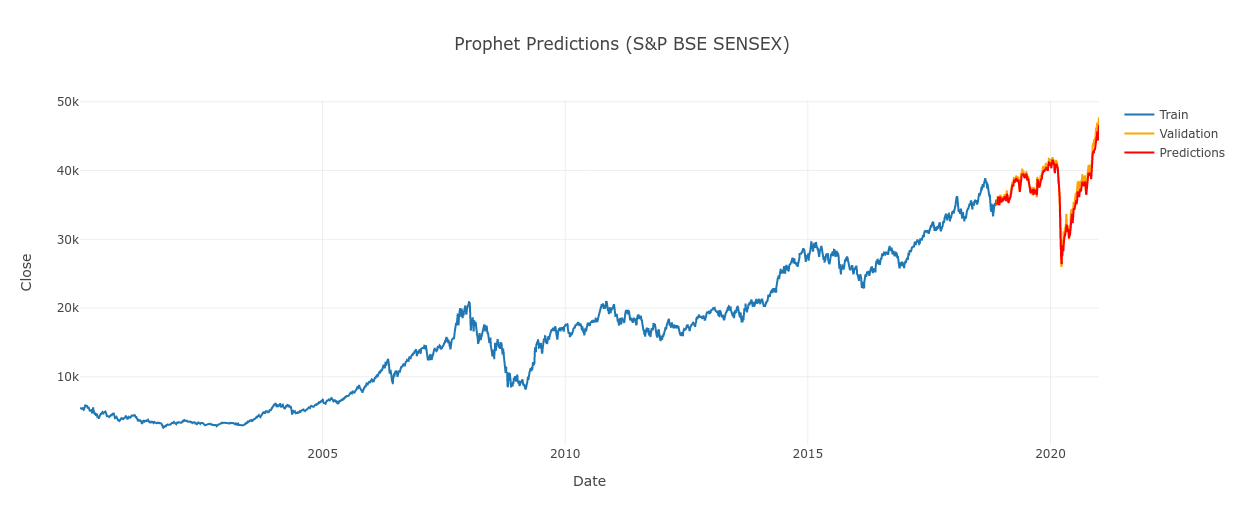
\includegraphics[width = \textwidth]{images/Prophet-SENSEX-Predictions.png}
		\caption{Prophet Model Predictions for Validation Data (S\&P BSE SENSEX).}
		\label{fig:my_label}
	\end{figure}
\end{frame}

\begin{frame}{SARIMAX and Prophet Predictions Combined (S\&P BSE SENSEX)}
	\begin{figure}
		\centering
		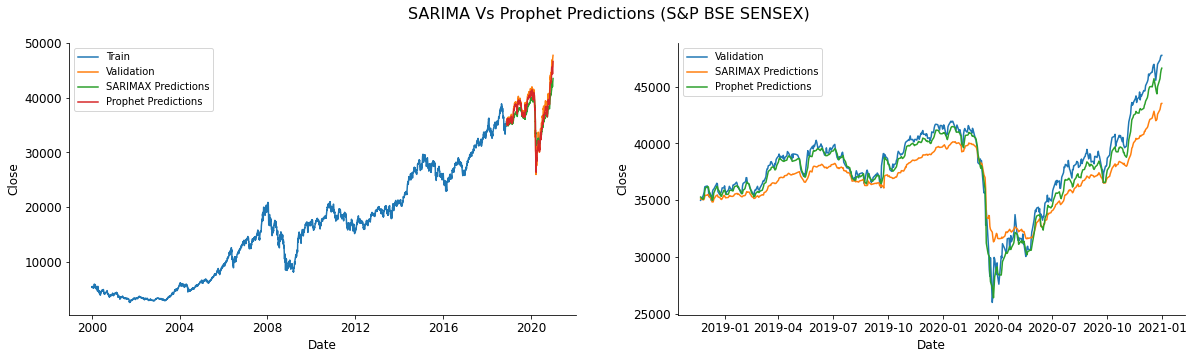
\includegraphics[width = \textwidth]{images/SARIMAX-Prophet-SENSEX-Predictions.png}
		\caption{Prophet and SARIMAX Predictions on S\&P BSE SENSEX Validation Set.}
		\label{fig:my_label}
		\pause
	\end{figure}
	\begin{table}[]
		\centering
		\begin{tabular}{c c c c c c}
			\textbf{Model} & \textbf{MAE} & \textbf{MSE}          & \textbf{RMSE} & \textbf{R2-Score} & \textbf{MAPE} \\
			\toprule
			SARIMAX        & 1553.135     & $3.386 \times 10^{6}$ & 1839.904      & 0.731307          & $4.05 \%$     \\
			Prophet        & 611.323      & $5.998 \times 10^{5}$ & 774.435       & 0.953             & $1.60\%$      
			\bottomrule
		\end{tabular}
		\caption{SARIMAX and Prophet Error Metric Values.}
		\label{tab:my_label}
	\end{table}
\end{frame}

\begin{frame}{Notes on Parameters of SARIMAX Model for S\&P-500}
	\begin{itemize}
		\item Estimated hyperparameters of SARIMAX$(p, d, q) \times (P, D, Q, M)$ are: \textbf{SARIMAX} $(5, 1, 1) \times (2, 0, 1, 7)$ with an AIC=$35701.260$.
	\end{itemize}
	\begin{figure}
		\centering
		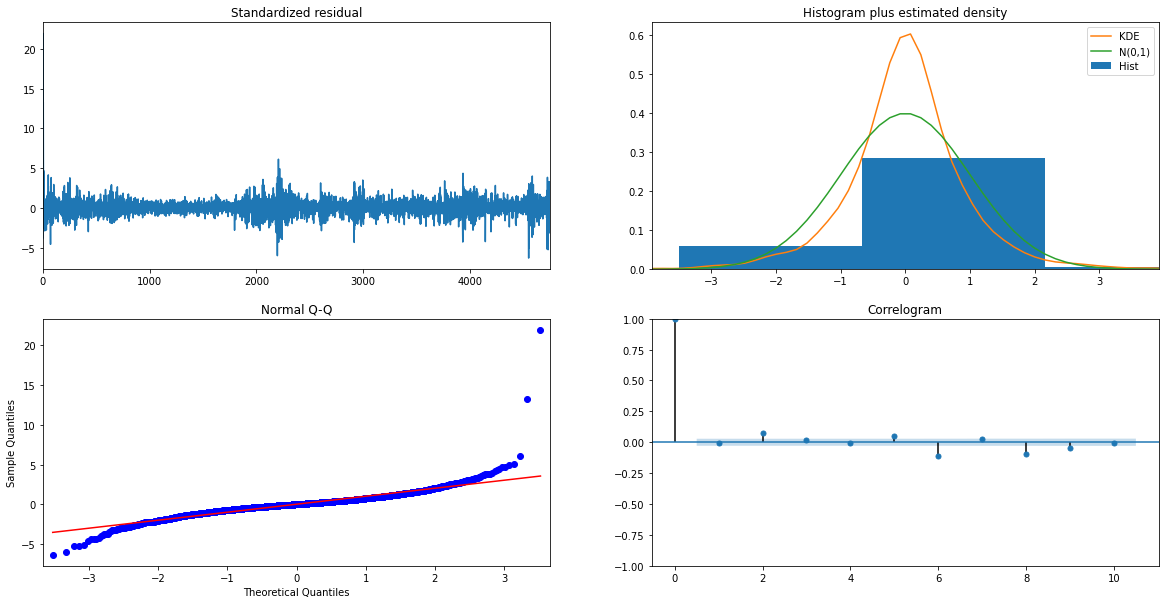
\includegraphics[width = \textwidth]{images/S&P-500 Auto ARIMA Training Results.png}
	\end{figure}
\end{frame}

\begin{frame}{SARIMAX Performance on Validation Set (S\&P-500)}
	\begin{figure}
		\centering
		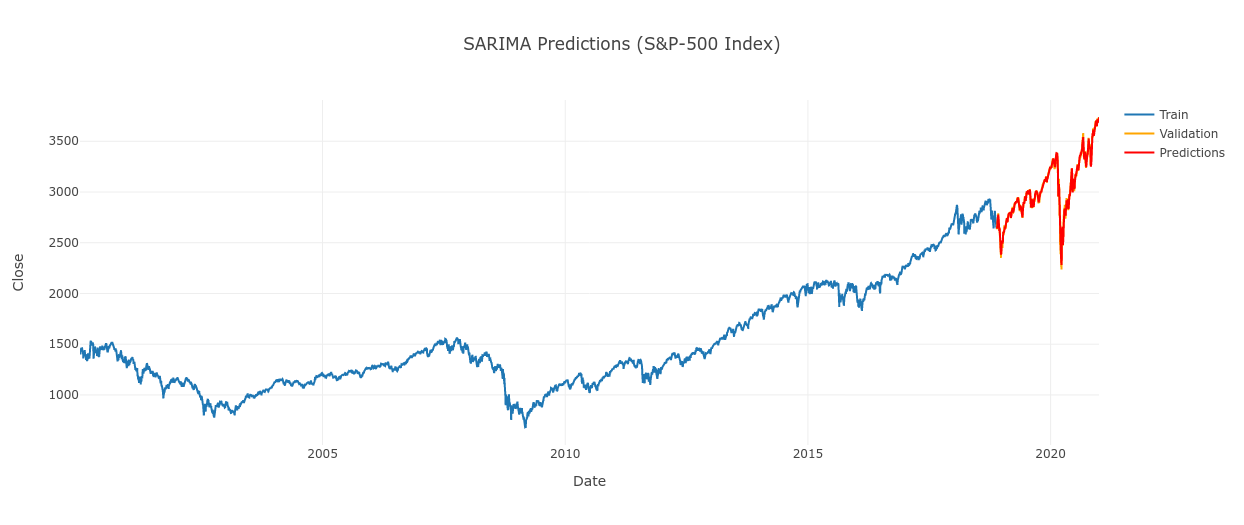
\includegraphics[width = \textwidth]{images/SARIMA S&P-500 Index Predictions.png}
		\caption{SARIMA Model Predictions for Validation Data (S\&P-500).}
		\label{fig:my_label}
	\end{figure}
\end{frame}

\begin{frame}{Prophet Performance on Validation Set (S\&P-500)}
	\begin{figure}
		\centering
		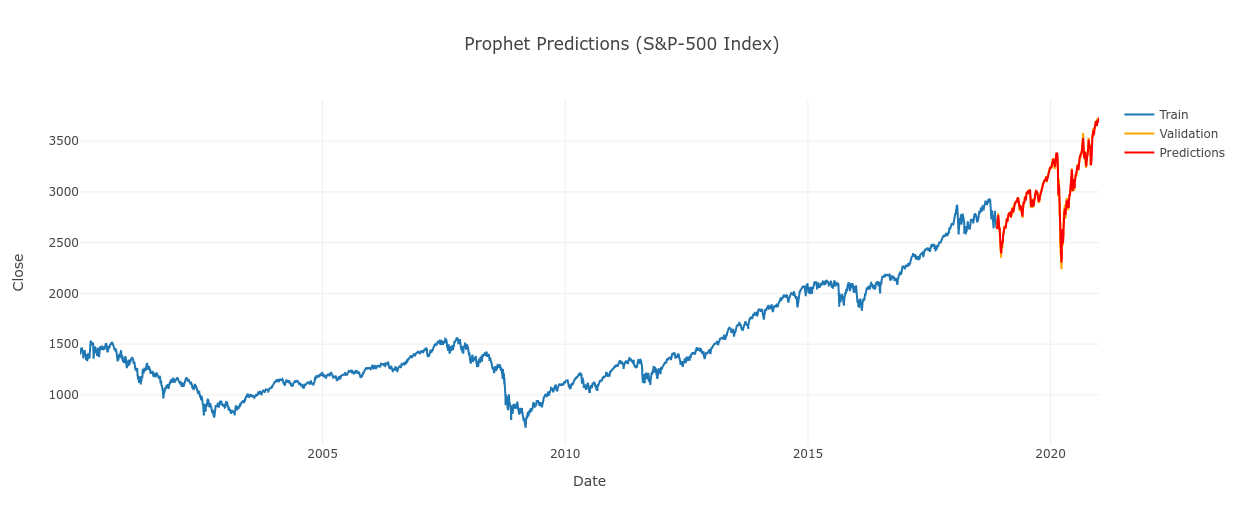
\includegraphics[width = \textwidth]{images/Prophet S&P-500 Predictions.png}
		\caption{Prophet Model Predictions for Validation Data (S\&P-500).}
		\label{fig:my_label}
	\end{figure}
\end{frame}

\begin{frame}{SARIMAX and Prophet Predictions Combined (S\&P-500)}
	\begin{figure}
		\centering
		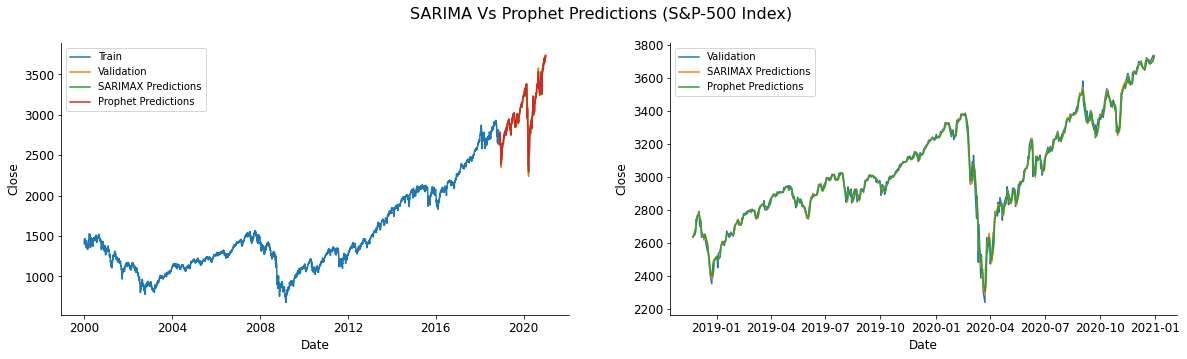
\includegraphics[width = \textwidth]{images/SARIMAX-Prophet-S&P-500-Predictions.png}
		\caption{Prophet and SARIMAX Predictions on S\&P-500 Validation Set.}
		\label{fig:my_label}
		\pause
	\end{figure}
	\begin{table}[htbp]
		\centering
		\begin{tabular}{c c c c c c}
			\textbf{Model} & \textbf{MAE} & \textbf{MSE} & \textbf{RMSE} & \textbf{R2-Score} & \textbf{MAPE} \\
			\toprule
			SARIMAX        & 18.189       & 755.416      & 27.484822     & 0.991685          & $0.62 \%$     \\
			Prophet        & 18.452       & 770.787      & 27.764        & 0.991516          & $0.63\%$      
			\bottomrule
		\end{tabular}
		\caption{SARIMAX and Prophet Error Metric Values.}
		\label{tab:my_label}
	\end{table}
\end{frame}

\section{Findings from the Study}
\begin{frame}{Findings from the Study}
	\begin{itemize}
		\item The volatility which was obeserved during the Global Financial Crisis of 2008, the same kind of volatility was observed in the COVID Crash of 2020 in both the markets i.e. USA and India.
		      \pause
		\item The markets independent of geography not only tells us the sentiment of the investor in short-term but also gives us an idea about what are the variables which plays a major role like budget annoucements, stimulus plans, FDIs etc to move the market in either directions, but in long term only those stocks/equities/securities performed well which represents high quality businesses.
		      \pause
		\item Both the markets i.e. Developed \& Emerging markets have rebounded quickly i.e. in approximately 7 months after the COVID-19 crash which itself is a thing to discuss because normally it takes atleast 2 years for the markets to recover to its early highs.
	\end{itemize}
\end{frame}

\section{Conclusions}
\begin{frame}{Conclusions}
	\begin{itemize}
		\item In this analysis, \textbf{SARIMAX$(2, 0, 0) \times (2, 0, 0, 7)$} for S\&P BSE SENSEX and \textbf{SARIMAX$(5, 1, 1) \times (2, 0, 1, 7)$} for S\&P-500 yielded a highly accurate results with a MAPE of $4.05\%$ and $0.61\%$.
		      \pause
		\item Prophet has performed better than both the ARIMA models when forecasting S\&P BSE SENSEX and S\&P-500 with MAPE of $1.06\%$ and $0.62\%$.
		      \pause
		\item This model can be used as a techinical indicator of what values the indexes would take in short term in order manage the portfolios to maximize the profits in the market.
	\end{itemize}
\end{frame}

\section{Future Work}
\begin{frame}{Future Work}
	\begin{itemize}
		\item In addition to forecasting the closing price, it will also be more strategic if we can also forecast the $\beta$ value i.e. measure of risk with respect to benchmark indices or broader market indices \cite{challa_malepati_kolusu_2018}.
		      \pause
		\item Adding more exogenous variables like P/E ratio, P/B ratio, Market Capitalisation etc as external features in the dataset can help in better forecasting.
	\end{itemize}
\end{frame}

\section{References}
\begin{frame}{References}
	\printbibliography
\end{frame}

\begin{frame}
	\Huge{\centerline{\textbf{Thank You}}}\\
	\footnotesize{\centerline{(The sildes were created using \LaTeX.)}}\\
	\small{\centerline{For Interactive Plots refer Google Colab Notebook}}
	\newline
	\small{\centerline{Notebook Link: \href{https://tinyurl.com/uvs7drpa}{https://tinyurl.com/uvs7drpa}}}
\end{frame}

\end{document}